\documentclass[12pt,a4paper]{article}
\usepackage[czech]{babel}
\usepackage{graphicx}
\usepackage{tabularx}
\usepackage{hyperref}
\usepackage[utf8]{inputenc}
\usepackage[T1]{fontenc}
\pagenumbering{gobble}
\setlength{\parskip}{1ex plus 0.5ex minus 0.2ex}
\setlength{\parindent}{0pt}
\usepackage[final]{pdfpages}

\parindent=2.2em

\pagestyle{empty}

% ~~~~~ POZICOVÁNÍ ~~~~~
% ~~ okraje
\global\newdimen\OKRAJE
\global\OKRAJE =2cm
% ~~ šířky
\setlength\textwidth{\paperwidth-2\OKRAJE}
\global\newdimen\DOKUMENTVYSKA
\setlength\oddsidemargin{(\paperwidth-\textwidth)/2 - 1in}
% ~~ výšky
\setlength{\DOKUMENTVYSKA}{\paperheight-2\OKRAJE}
\setlength{\headsep}{0pt}
\setlength\topmargin{(\paperheight-\DOKUMENTVYSKA)/2 - 3.7cm}
\setlength\textheight{\DOKUMENTVYSKA}
% ~~ „Anglické“ odstavce
\setlength\parskip{5px}
\setlength\parindent{0cm}


%~~~~~~~~~~~~~~~~~~~~~~~~~~~~~~~~~~~~~~~
\def\endmp{\\[-5px]}
\def\begmp{\ \\[-10px]}
\def\asize{1.5cm}
\def\bsize{6cm}

%~~~~~~~~~~~~~~~~~~~~~~~~~~~~~~~~~~~~~~~
%~~~~~~~~~~~~DOKUMENT~~~~~~~~~~~~~~~~~~~
%~~~~~~~~~~~~~~~~~~~~~~~~~~~~~~~~~~~~~~~

\begin{document}
\title{Chinin}
\author{Jiří Kalvoda}
\date{}
\maketitle
\begin{minipage}[t]{0.5\textwidth}
	\begin{center}

		{\Large Chinovník} (Cinchona)\\[10px]

		\includegraphics[width=4cm]{1.jpg}

	\end{center}
	\begin{itemize}
		\item stromy nebo keře
		\item vstřícné listy a pětičetné květy
		\item Tropická Amaerika (Kostarika -- Bolívie)
		\item chinovník lékařský a chinovník pýřitý
		\item $7\%$ až $16\%$ chninu v kůře
	\end{itemize}
\end{minipage}
\begin{minipage}[t]{0.5\textwidth}
	\begin{center}

		{\Large Remijia}\\[10px]

		\includegraphics[width=4cm]{2.jpg}

	\end{center}
	\begin{itemize}
		\item keře a stromy
		\item velké vstřícné nebo přeslenité listy
		\item bílé až červené květy
		\item Pouze v J. Americe (Amazonii)
		\item $0.5\%$ až $2\%$ chninu v kůře
	\end{itemize}

\end{minipage}\\[20px]

\begin{minipage}{0.5\textwidth}
	\begin{center}
		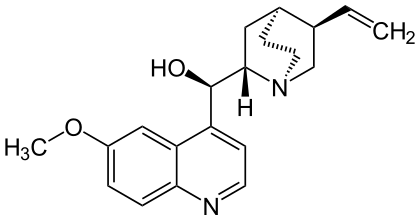
\includegraphics[width=7cm]{3.jpg}
	$\rm C_{20}H_{24}N_2O_2$
	\end{center}
\end{minipage}
\begin{minipage}{0.5\textwidth}

	\begin{itemize}
		\item rozpustný v ethanolu; špatně ve vodě
		\item v UV světle fluoreskuje
		\item bílý prášek
		\item zásadité vlstnosti
	\end{itemize}
\end{minipage}\\[20px]

\begin{minipage}{0.5\textwidth}
	\begin{itemize}
		\item slabé analgetikum, antipyretikum
		\item lék proti malárii
		\item součástí alkoholických nápojů a toniků
		\item krémy a šamóny
		\item gumárenský průmysl: vulkanizační prostředek
	\end{itemize}
\end{minipage}
\begin{minipage}{0.5\textwidth}
	\begin{itemize}
		\item hořká chuť
		\item povzbuzuje chuť k jídlu
		\item spomaluje srdce, snižuje krevní tlak
		\item smrtelná dávka pro člověka je 8-10 gramů
	\end{itemize}
\end{minipage}
\end{document}
